\section{Structure et organisation des génomes procaryotes}
\label{sec:structure_org}

%Le génome correspond à l'ensemble du matériel génétique, c.-à-d., des éléments qui seront hérités par les cellules de la génération suivante. Le génome, c'est aussi la structure de base qui va contenir l'ensemble des informations nécessaires au fonctionnement et à la survie de la cellule. Ces informations sont contenues dans la molécule d'ADN, ce qui nous amène à la structure primaire du génome, la séquence nucléotidique. Cette séquence est souvent circulaire chez les procaryotes et est de petite taille, quelques centaines de milliers de bases, mais certains génomes peuvent atteindre plusieurs millions de bases\footnote{En bioinformatique, on utilise l'unité base (b) ou paire de base (pb), pour mesurer la taille d'un génome. Un génome procaryote sera donc compris entre 100 kb et 10 Mb. Pour comparaison, le génome humain mesure environs 3 Gb.} (\autoref{fig:genome_size}).

Le génome procaryote correspond à la séquence de nucléotides qui composent la molécule d'ADN qui est bicaténaire, \textit{i.e.}, composée de deux brins antiparallèles reliés par complémentarité des bases (A$\leftrightarrow$T, C$\leftrightarrow$G). Le génome est souvent circulaire et de petite taille, quelques centaines de milliers de bases, mais certains génomes peuvent atteindre plusieurs millions de bases\footnote{En bioinformatique, on utilise l'unité base (b) ou paire de base (pb), pour mesurer la taille d'un génome. Un génome procaryote sera donc compris entre 100 kb et 15 Mb. Pour comparaison, le génome humain mesure environs 3 Gb.} (\autoref{fig:genome_size}). Enfin, le génome se divise en deux grandes catégories : l'ADN codant et l'ADN non codant.

\begin{figure}[htbp]
    \centering
    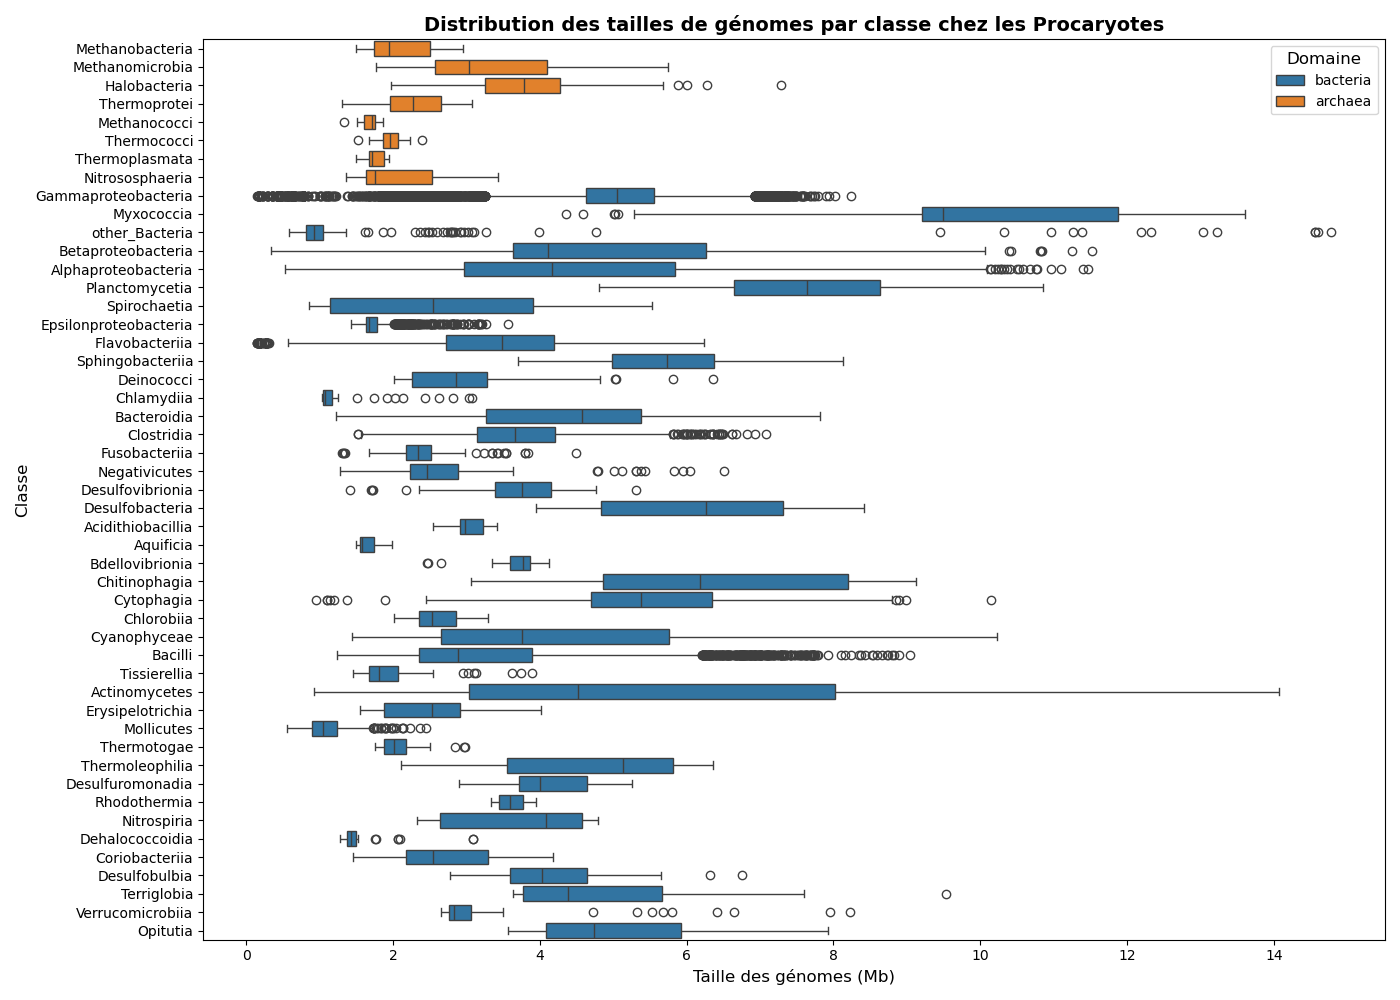
\includegraphics[width=\textwidth]{images/genome_sizes_boxplot.png}
    \caption[Distribution de la taille des génomes chez les procaryotes]{Distribution de la taille des génomes (en base) par classe chez les procaryotes. Les données utilisées proviennent de RefSeq version 28 janvier 2025.}
    \label{fig:genome_size}
\end{figure}

\newpage
\subsection{Constituant du génome : le codant et le non codant}
\label{sec:gene}
%\subsection{Organisation génique des procaryotes}
Chez les procaryotes, le génome est majoritairement constitué de séquences codantes (entre 85 et 90 \%), ce qui compense leur petite taille. 
L'ADN codant correspond à des blocs de nucléotides d’environ 1 kb. Ces blocs codants sont appelés gènes et ils jouent un rôle essentiel puisqu’ils contiennent l’information nécessaire à la production des protéines impliquées dans toutes les réactions cellulaires (cf. \autoref{sec:fn_reg}). De plus, l’ADN procaryote étant bicaténaire, chaque gène peut alors être lu dans les deux directions (sur le brin direct ou complémentaire), doublant ainsi la quantité d'information sur une position précise du génome (locus). 

Dans le génome, les gènes ne sont pas répartis aléatoirement. Ceux qui codent une fonction biologique similaire sont souvent regroupés dans un  contexte génomique. La conservation de l'ordre des gènes, appelé aussi synténie, peut varier entre les génomes, mais les gènes restent dans le même contexte \cite{lathe_gene_2000}, on parle alors de contexte conservé ou de synténie conservée. De plus, la position des gènes par rapport à l'origine de réplication (Ori: région où commence la réplication de l'ADN) à aussi son importance. Il a été montré que chez les bactéries avec un fort taux de division, les gènes ayant un rôle essentiel sont plus proches de l'Ori afin d'être plus fortement exprimés \cite{sharp_chromosomal_1989,vieira-silva_systemic_2010}.
%Les gènes sont soumis à des mécanismes de régulation communs (cf. \autoref{sec:fn_reg}).

Pour finir, les gènes peuvent être classés selon l’importance de leur fonction pour la survie de la cellule. Les gènes indispensables au cycle de vie d'une cellule, par exemple la réplication de l’ADN, la transcription, ou la traduction, sont dits "essentiel" et se distinguent des gènes "accessoires", qui codent pour des fonctions d'adaptation à des conditions particulières, comme la résistance aux antibiotiques, la défense contre les virus ou des transformations métaboliques spécifiques.



%Le génome est divisé en sous-unité que l'on appelle gène. Le gène contient l'information nécessaire pour produire une protéine qui réalisera une fonction dans la cellule (\autoref{fig:gene2prod}), on dit que le gène code pour une protéine. Pour ça, l'ADN est d'abord transcrit en une molécule d'ARNm, qui sera traduite en protéine (gène A sur la \autoref{fig:genome_size}) par des complexes protéine/ARN, les ribosomes. Ces protéines correspondent à une chaîne d'acides aminés, que l'on peut représenter sous forme de séquence. Pour passer d'un gène à une protéine, on utilise une table de correspondance que l'on appelle code génétique où 3 nucléotides correspondent à 1 acide aminé. En moyenne, une protéine contient 300 acides aminés, ramenant la taille des gènes à environ 1 kb. Enfin, comme indiqué sur la partie haute de la \autoref{fig:genome_size}, les génomes procaryotes sont majoritairement codants, ce qui veut dire que presque tout l'ADN peut être divisé en gènes, et donc qu'il y a environ entre 100 et 10 000 gènes dans les génomes en fonction de leur taille. En mettant toutes ces informations en perspective, on comprend que la petite taille des génomes procaryotes est compensée par son fort taux de gènes, et qu'ainsi, il contient l'ensemble des protéines nécessaires à la survie de la cellule. 


\begin{figure}[htbp]
    \centering
    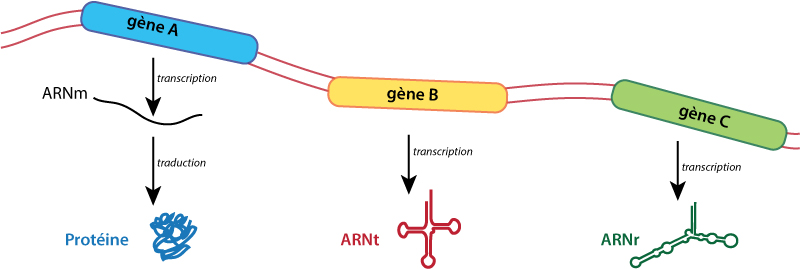
\includegraphics[width=\linewidth]{images/gene2prot.jpg}
    \caption[Produit d'un gène]{Produit d'un gène dans la cellule. Un gène est d'abord transcrit en ARN. Si l'ARN transcrit est dit messager (ARNm), il sera ensuite traduit en protéine, sinon l'ARN produit (ARNt, ARNr, miARN, ....) aura un rôle spécifique dans des processus cellulaire. Copié de RNBio, Sorbonne université. \url{https://rnbio.sorbonne-universite.fr/genetique_genotype1}}
    \label{fig:gene2prod}
\end{figure}

L'ADN non codant constitue une part tout de même importante du génome et selon l'adage "la nature a horreur du vide"\footnote{Citation d'Aristote qui, répondant à Démocrite, dit que l'univers ne pouvait être rempli de vide. On sait aujourd'hui que Démocrite avait raison, mais dans le cas des génomes procaryote, l'idée fonctionne.}. Cet ADN non codant, n'est donc pas inutile et renferme également des fonctions essentielles à la vie de la cellule.
Tout d'abord, on retrouve les séquences d'ADN qui seront transcrits en ARN ribosomiques (ARNr) ou ARN de transfert (ARNt). Ces ARN sont indispensables pour la construction de la chaîne d'acide aminée de la protéine. Ces séquences d'ADN sont considérée aussi comme des gènes et selon les sources comme faisant partie du codant. Cependant, d'un point de vue sémantique et biologique ces gènes ne code pas, les nucléotides sont copiés d'une forme d'acide désoxyribonucléique en une forme d'acide ribonucléique. L'ADN non codant renferme d'autres formes d'ARN, comme les microARN et les ARN interférents (miARN et siARN). Ces ARN sont aujourd'hui considérés comme des acteurs clés dans la régulation des fonctions biologiques \cite{backofen_bioinformatics_2014,watkins_regulatory_2019}, mais aussi dans d'autres processus comme le système immunitaire \cite{bobadilla_ugarte_argonaute_2023}.

L'ADN non codant n'a pas uniquement le rôle de contenir les séquences transcrites en ARN, il contient aussi d'autres éléments régulateurs de l'expression des gènes contenus dans l'espace intergénique (cf. \autoref{sec:fn_reg}). On retrouve aussi dans l'ADN non codant des séquences répétées, comme les séquences d'insertion (IS) qui se déplace dans le génome, ou les séquence CRISPR (Régions composées de répétitions palindromiques et d’espacers, impliquées dans le système immunitaire adaptatif des bactéries) \cite{jansen_identification_2002,bolotin_clustered_2005}. Il existe tout de même une partie d'ADN non codant qui n'a aucun rôle, ces séquences sont des vestiges d'anciens gènes qui au cours de l'évolution ont perdu leur fonction (cf. \autoref{sec:dyn_evo}). Pour terminer, c'est aussi dans le non-codant que l'on va retrouver des éléments essentiels dans la réplication et l'évolution des génomes procaryotes : l'origine de réplication (Ori) et les éléments génétique mobile (MGE). 
%Tous les gènes ne sont pas traduits en protéine, une partie de ces gènes seront transcrit dans des formes d'ARN ayant un rôle dans la régulation et le fonctionnement de la cellule. Les ARN ribosomiques (ARNr), sont les constituants fondamentaux de la structure et du fonctionnement des ribosomes. Ils vont interagir avec les ARN de transfert (ARNt), qui acheminent les acides aminés vers les ribosomes pour traduire l'ARNm en protéine. D'autres ARN, comme les microARN et les ARN interférents (miARN et siARN), interviennent dans la régulation de l'expression des gènes. Cette liste non exhaustive montre la diversité des ARN et beaucoup étaient encore considérés il y a peu comme des produits secondaires sans réelle fonction. Aujourd'hui, ils sont considérés comme des acteurs clés dans la régulation des fonctions biologiques \cite{watkins_regulatory_2019,backofen_bioinformatics_2014}, mais aussi dans d'autres processus comme le système immunitaire \cite{bobadilla_ugarte_argonaute_2023}

\subsection{Réplicons et mécanismes de réplication dans les génomes procaryotes}
\label{sec:replicons}
La multiplication des cellules procaryotes s'effectue par division, où une cellule mère donne naissance à deux cellules filles. Afin de transmettre l’information génétique aux cellules nouvellement formées, l’ADN doit être répliqué, \textit{i.e.}, copié de manière exacte. Le terme réplicon désigne l’ensemble des molécules d’ADN capables de se répliquer de façon autonome. Un réplicon contient ainsi tous les éléments nécessaires à l’exécution et à la régulation de la réplication. Chaque réplicon contient une séquence d’ADN spécifique, appelée origine de réplication (Ori), où commence le processus de réplication.

La forme principale de réplicon dans la cellule procaryote est le chromosome. Le chromosome, souvent circulaire et replié, constitue le plus grand réplicon en termes de paires de bases. Chez les procaryotes, le chromosome est généralement unique, bien que d'autres réplicons puissent coexister au sein de la cellule.

Une seconde forme de réplicon, connue pour son rôle dans l’évolution (voir \autoref{sec:evo_hz}), est le plasmide \cite{lederberg_gene_1946,lederberg_sex_1953}. Les plasmides, souvent circulaires et de taille inférieure à celle du chromosome, sont indépendants de ce dernier. En tant que réplicons, ils se répliquent de manière autonome et peuvent être présents en grand nombre dans une cellule. L’origine de réplication des plasmides diffère de celle des chromosomes. Par ailleurs, les plasmides peuvent accumuler de nouvelles séquences et augmenter en taille, prenant alors la forme de mégaplasmides (\autoref{fig:replicon}).

Chez la majorité des procaryotes, le chromosome contient les gènes essentiels, tandis que les plasmides portent des gènes accessoires. Cependant, certaines formes de réplicons oscillent entre chromosome et plasmide. Par exemple, chez \textit{Rhodobacter sphaeroides}\footnote{Bactérie présente dans les lacs profonds et les eaux stagnants. Elle est capable de réaliser la photosynthèse et son métaolisme est très diversifié et donc très utilisé en biotechnologie} et \textit{Vibrio cholerae}\footnote{Bactérie responsable du choléra, on la retrouve dans l'eau et peut se propager entre humain en utilisant la transpiration}, un second chromosome a été identifié \cite{suwanto_physical_1989,trucksis_vibrio_1998}. Aujourd'hui, ces chromosomes secondaires sont distingués d'une forme de réplicons proche, le chromide \cite{harrison_introducing_2010}. Les chromides, de taille intermédiaire entre un plasmide et un chromosome principal, contiennent des gènes essentiels à la cellule. Ces gènes présentent une proximité phylogénétique avec les espèces du même genre, contrairement à ceux du chromosome principal, qui sont conservés au-delà du genre. En revanche, en termes de mécanismes de réplication et de séquences Ori, les chromids utilisent des systèmes de type plasmidique.

L’usage des termes chromosome secondaire, chromid et mégaplasmide demeure actuellement peu standardisé dans la littérature \cite{hall_what_2021}. Plusieurs critères permettent néanmoins de les distinguer. Le premier repose sur le contenu génétique : les mégaplasmides n’abritent pas de gènes essentiels, contrairement aux chromosomes secondaires et aux chromids. Le second critère est la composition en nucléotides, qui est plus proche de celle du chromosome principal pour les chromids et les chromosomes secondaires. Enfin, leur origine évolutive les différencie : le chromosome secondaire résulte de la scission d’un chromosome ancestral en un chromosome principal et un secondaire, tandis que le chromid dérive d’un ancien mégaplasmide ayant perdu sa capacité de mobilité (voir \autoref{sec:evo_hz}) et qui a intégré des gènes essentiels (\autoref{fig:replicon}). Les chromides auraient donc plutôt un rôle de réservoir de gènes d'intérêt et d'adaptation améliorant la \textit{fitness} des organismes. Cette vision vertueuse de l'accumulation de gènes s'oppose directement à la vision plus ancienne des plasmides non mobilisable décrits comme parasitant la cellule \cite{levin_accessory_1993,lili_persistence_2007}.

\begin{figure}[htbp]
    \centering
    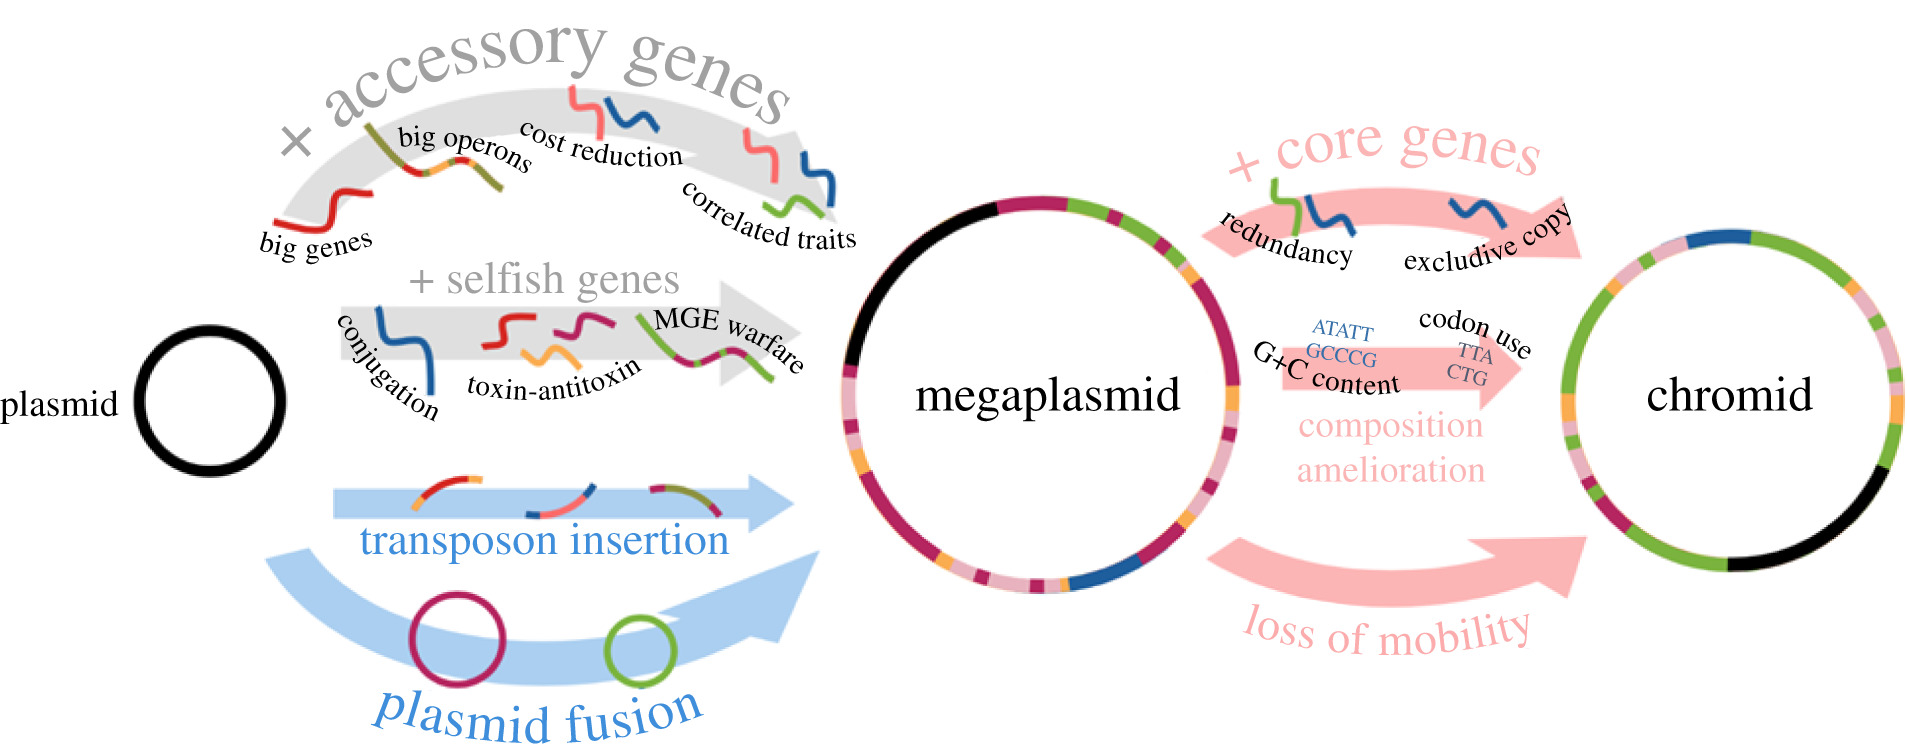
\includegraphics[width=0.8\linewidth]{images/replicon.jpg}
    \caption[Évolution d'un plasmide en chromid]{Schéma simplifié de l'évolution d'un plasmide en megaplasmide et de megaplasmide à chromid. Figure extraite de \cite{hall_what_2021}}
    \label{fig:replicon}
\end{figure}

